\documentclass[11pt,oneside,a4paper]{book}
\usepackage[%
  a4paper,%
  left = 20mm,%
  right = 20mm,%
  textwidth = 178mm,%
  top = 40mm,%
  bottom = 30mm,%
  %heightrounded,%
  headheight=70pt,%
  headsep=25pt,%
]{geometry}
\usepackage{graphicx}
%\usepackage[sfdefault,light]{Helvetica}
\usepackage[sfdefault,light]{FiraSans}
\usepackage{titlesec}
\usepackage{hyperref}
\hypersetup{
    colorlinks = true,
    allcolors  = link-blue, 
}
\usepackage{lastpage}
\usepackage{graphicx}
\usepackage{float}
\usepackage{xspace}
\usepackage{longtable}
\usepackage{tabularx}
\usepackage{color,colortbl}
\usepackage{longtable} % Paquete para tablas largas
\usepackage{colortbl}  % Colores en tablas
\usepackage[table,xcdraw]{xcolor} % Colores adicionales


\definecolor{link-blue}{RGB}{6,69,173}
\definecolor{dark-green}{RGB}{52,133,62}
\definecolor{light-blue}{RGB}{127,180,240}
\definecolor{dark-blue}{RGB}{72,120,224}
\definecolor{heading-grey}{RGB}{128,128,128}
\definecolor{heading2-grey}{RGB}{200,200,200}
\definecolor{Critical}{RGB}{192,0,0}
\definecolor{High}{RGB}{255,0,0}
\definecolor{Medium}{RGB}{255,192,0}
\definecolor{Low}{RGB}{255,255,0}
\definecolor{Informational}{RGB}{94,185,255}

\usepackage{listings}
\usepackage{enumitem}
\usepackage{array,booktabs}
\usepackage{fancyhdr}
\renewcommand{\footrulewidth}{0.2pt}
\renewcommand{\headrulewidth}{0.2pt}
\fancyfoot{}
\fancyhead{}
\fancyfoot[C]{Confidential}
\fancypagestyle{plain}{
    \fancyfoot[R]{\\ \textcolor{heading-grey}{\newline Página \thepage\ de \pageref{LastPage}}}
    \fancyfoot[C]{\textcolor{heading-grey}{\textbf{Proyecto de Fin de Ciclo -- \projectno}  }}
    \fancyhead[R]{
\includegraphics[width=1cm]{img/logo.jpg}}
}
\fancypagestyle{fancy}{
    \fancyfoot[R]{\\ \textcolor{heading-grey}{\newline Página \thepage\ de \pageref{LastPage}}}
    \fancyfoot[C]{\textcolor{heading-grey}{\textbf{Proyecto de Fin de Ciclo -- \projectno}   }}
    \fancyhead{}
}
\thispagestyle{fancy}\pagestyle{plain}

\newcommand{\email}[1]{\href{mailto://#1}{#1}}
\newcommand{\newchapter}[1]{{\section*{#1}
\addcontentsline{toc}{chapter}{#1}}}
\newcommand{\newsection}[1]{{\subsection*{#1}
\addcontentsline{toc}{section}{#1}}}
\newcommand{\newsubsection}[1]{{\subsubsection*{#1}
\addcontentsline{toc}{subsection}{#1}}}
\usepackage[skip=10pt plus1pt, indent=0pt]{parskip}
\usepackage{float} % Añadir al preámbulo si no lo tienes

\usepackage{etoolbox}
\makeatletter
\patchcmd{\chapter}{\if@openright\cleardoublepage\else\clearpage\fi}{}{}{}
\makeatletter
\renewcommand\tableofcontents{%
    \if@twocolumn
      \@restonecoltrue\onecolumn
    \else
      \@restonecolfalse
    \fi
    \section*{\contentsname
        \@mkboth{%
           \MakeUppercase\contentsname}{\MakeUppercase\contentsname}}%
    \@starttoc{toc}%
    \if@restonecol\twocolumn\fi
    }
\makeatother


\titleformat{\section}
{\normalfont\huge\bfseries}{\thesection}{1em}{}
\titleformat{\subsection}
{\normalfont\Large\bfseries}{\thesubsection}{1em}{}
\titleformat{\subsubsection}
{\normalfont\large\bfseries}{\thesubsubsection}{1em}{}

% \titleformat{command}[shape]{format}{label}{sep}{before}[after]
% \titlespacing{command}{left spacing}{before spacing}{after spacing}[right]

\titlespacing{\section}{0pt}{1em}{0.5em}
\titlespacing{\subsection}{0pt}{0em}{0.25em}

\usepackage[T1]{fontenc}
\renewcommand*\oldstylenums[1]{{\firaoldstyle #1}}

\def\projectno{Cloud Privado Dinámico}


\usepackage[spanish]{babel}
\usepackage[utf8]{inputenc}
\usepackage[T1]{fontenc}


\newcommand{\blankpage}{
  \clearpage
  \begingroup
  \pagestyle{empty}
  \null
  \vfill
  \newpage
  \addtocounter{page}{-1} % ¡esto es clave!
  \endgroup
}

\begin{document}

\renewcommand{\headrulewidth}{0pt}

%%%%%%%%%%%%%%%%%%%%%%%%%%%%%%%%%%%%%%%%%
%%          Begin title page           %%
%%%%%%%%%%%%%%%%%%%%%%%%%%%%%%%%%%%%%%%%%

\begin{titlepage}
   \thispagestyle{fancy}
   \begin{center}
        \vspace*{8em}
   
        \centering
\includegraphics[width=13cm]{img/logo_iescierva.jpg}

        \vspace{3em}

        \huge{\textbf{Proyecto Final de Ciclo \\
        Cloud Privado Dinámico}}

        \vspace{8em}

        \Large{Moisés Tamaalit Martínez\\
        2º Administración de Sistemas Informáticos en Red}

        \vspace{4em}

        \normalsize{
            IES Ingeniero de la Cierva\\
            Curso 2024/2025
        }

   \end{center}
\end{titlepage}

\blankpage

\newpage

\tableofcontents
\blankpage
\newpage

%%%%%%%%%%%%%%%%%%%%%%%%%%%%%%%%%%%%%%%%%
%%           Begin contents            %%
%%%%%%%%%%%%%%%%%%%%%%%%%%%%%%%%%%%%%%%%%

\newchapter{Información de contacto}

\begin{table}[h]
\begin{center}
    \begin{tabular}{|m{5cm}|m{3cm}|m{7.5cm}|} % Anchos ajustados aquí
        \hline
        \rowcolor{heading-grey}\multicolumn{1}{|>{\centering\arraybackslash}m{5cm}|}{\textcolor{white}{\textbf{Nombre}}} & 
        \multicolumn{1}{>{\centering\arraybackslash}m{3cm}|}{\textcolor{white}{\textbf{Título}}} & 
        \multicolumn{1}{>{\centering\arraybackslash}m{7.5cm}|}{\textcolor{white}{\textbf{Contacto}}} \\ \hline
        Moisés Tamaalit Martínez & Alumno & Email: \href{mailto:moisestamaalit@gmail.com}{moisestamaalit@gmail.com} \\ \hline
    \end{tabular}
\end{center}
\end{table}


\newpage

\newchapter{Preámbulo}
Antes de todo, quisiera agradecer al \textbf{IES Ingeniero de la Cierva} por proporcionar los recursos e infraestructura necesarios para desarrollar este proyecto. Su apoyo constante y el acceso a equipamiento profesional han sido fundamentales para alcanzar los objetivos propuestos.

Gracias a \textbf{sys4net} por el aprendizaje y la inspiración que me han proporcionado. En este periodo de prácticas, he podido aplicar y ampliar mis conocimientos en administración de sistemas, lo que ha sido crucial para el desarrollo de este proyecto. La experiencia adquirida en un entorno profesional ha sido invaluable y me ha permitido enfrentar desafíos reales, mejorando mis habilidades técnicas y mi capacidad para resolver problemas.

Gracias a Cayetano por acompañarme como tutor en las RMSkills, Spainskills, Worldskills y próximamente Euroskills. Su apoyo y orientación han sido clave para la gran adquisición de conocimientos y habilidades que he desarrollado durante este tiempo.

Gracias a Alejandro, mi tutor de este proyecto, por las ideas y sugerencias que me ha proporcionado, al igual que por su orientación durante el desarrollo del proyecto.

Gracias a todos mis profesores de este ciclo formativo por toda la enseñanza que me han proporcionado durante estos dos años. Cada uno de ellos ha aportado su grano de arena, enseñándome técnicas, herramientas y conocimientos que han sido esenciales para mi formación como administrador de sistemas.

Un último agradecimiento a José Carmelo, quién en grado medio, hace casi cuatro años, despertó mi interés por la informática, por los sistemas alternativos a Windows, por las redes y todo este mundo. Su pasión por la tecnología y la docencia despertó mi motivación y me impulsó a llevarme a donde estoy hoy.

\blankpage

\newchapter{Resumen}
Este proyecto presenta el desarrollo de una plataforma de \textit{hosting} VPS que permite desplegar y gestionar servidores virtuales de forma automatizada. La solución implementa una arquitectura de microservicios moderna, usando React, Node.js y Python, ofreciendo una interfaz intuitiva para usuarios sin conocimientos técnicos avanzados.

Los objetivos principales incluyen la automatización del despliegue de VPS, monitorización en tiempo real y gestión simplificada de servidores. Los resultados demuestran una plataforma funcional que cumple estos objetivos, proporcionando una solución segura y escalable.

\newpage
\blankpage
\newchapter{Introducción}

\newsection{Contextualización}
En la actualidad, la demanda de servidores virtuales privados (VPS) ha aumentado significativamente debido a la creciente necesidad de infraestructura \textit{cloud} flexible y escalable. Las empresas y desarrolladores buscan soluciones que les permitan desplegar y gestionar recursos de forma eficiente.

\newsection{Justificación}
La elección de este proyecto se basa en:
\begin{itemize}
    \item Experiencia previa en administración de sistemas.
    \item Interés en tecnologías de virtualización.
    \item Identificación de la necesidad de soluciones más accesibles.
    \item Oportunidad de aplicar conocimientos del ciclo formativo.
    \item Oportunidad de aprender sobre desarrollo web y de APIs.
\end{itemize}


\newsection{Objetivos del Proyecto}
\textbf{Principales:}
\begin{itemize}
    \item Desarrollar una plataforma completa de gestión de VPS.
    \item Automatizar el despliegue de servidores virtuales.
    \item Implementar monitorización en tiempo real.
\end{itemize}

\textbf{Secundarios:}
\begin{itemize}
    \item Crear una interfaz de usuario intuitiva.
    \item Optimizar el rendimiento del sistema.
    \item Documentar el proceso de desarrollo.
\end{itemize}

\newpage
\blankpage
\newsection{Alcance}
El proyecto abarca el desarrollo de una plataforma de \textit{hosting} VPS que incluye:
\begin{itemize}
    \item Interfaz web para usuarios.
    \item API para gestión de VPS.
    \item Integración con Proxmox VE como hipervisor.
    \item Sistema de autenticación y autorización.
    \item Monitorización de recursos en tiempo real.
\end{itemize}
El sistema está diseñado para ser escalable y adaptable a diferentes necesidades, permitiendo la incorporación de nuevas funcionalidades en el futuro.

\newpage
\blankpage
\newchapter{Análisis previo}
\newsection{Necesidades detectadas}
El mercado actual de \textit{hosting} VPS presenta una barrera significativa para usuarios sin experiencia técnica avanzada. Los paneles de control existentes suelen ser complejos y poco intuitivos, dificultando la gestión de servidores virtuales. Además, la automatización del despliegue y configuración de VPS es limitada, requiriendo frecuentemente intervención manual.

\newsection{Requisitos técnicos y funcionales}
Los requisitos técnicos incluyen un servidor Proxmox VE como base de virtualización, mínimo 32GB de RAM y procesador con soporte para virtualización (Intel VT-x o AMD SVM). 

La plataforma debe soportar múltiples usuarios concurrentes y garantizar el aislamiento de recursos. 

Funcionalmente, se requiere una interfaz web amigable con el usuario, sistema de autenticación seguro, panel de control intuitivo y monitorización en tiempo real de recursos.

\newsection{Herramientas y tecnologías}
Para desarrollar el proyecto, se ha usado un servidor \textbf{HPE Proliant DL360 Gen9} con \textbf{80GB de RAM}, 2 procesadores \textbf{Intel Xeon E5-2680 v3} y almacenamiento mixto \textbf{HDD/SSD}. Este servidor se encuentra alojado en el centro de datos del IES Ingeniero de la Cierva, lo que permite un acceso rápido y seguro a los recursos.

La implementación se basa en React con TypeScript para el \textit{frontend}, proporcionando una experiencia de usuario moderna y \textit{responsive}. El \textit{backend} utiliza Node.js con Express para la API principal, mientras que Python con FastAPI gestiona la interacción con Proxmox. MariaDB sirve como base de datos relacional, y Docker facilita la contenerización de servicios. Proxmox VE actúa como hipervisor base.

La memoria y documentación del proyecto es escrita en LaTeX, lo que permite una presentación profesional y estructurada de la información. Los diagramas se han realizado con Draw.io, una herramienta en línea que facilita la creación de diagramas y esquemas; y dbdiagram.io para el esquema de la base de datos.

\newsection{Estudio de viabilidad}
El análisis de viabilidad indica que el proyecto es técnicamente factible con los recursos disponibles. Los costes se limitan principalmente al hardware necesario para el servidor Proxmox en este entorno. 

En un entorno de producción, hay que sumarle el coste de un bloque de IPs, los dominios que fueran a usarse y el mantenimiento del servidor. 

El tiempo estimado de desarrollo es de 4 meses, considerando las fases de diseño, implementación y pruebas. 

Los riesgos principales incluyen la complejidad de la integración con Proxmox y la necesidad de optimizar el rendimiento del sistema.

\newpage
\blankpage

\newchapter{Metodología}

\newsection{Frontend (React + TypeScript)}
Para el desarrollo del frontend se ha utilizado \textbf{React 19} con \textbf{TypeScript}, lo que permite crear una interfaz de usuario moderna y escalable.

\textbf{React} es una biblioteca de JavaScript para construir interfaces de usuario, mientras que \textbf{TypeScript} es un superconjunto de JavaScript que añade tipado estático, lo que mejora la calidad del código y facilita el mantenimiento a largo plazo.

La ventaja de usar React es su capacidad para construir componentes reutilizables y su ecosistema robusto. TypeScript añade tipado estático, mejorando la mantenibilidad del código y reduciendo errores en tiempo de ejecución.

Se ha implementado \textbf{Tailwind CSS} para estilos y \textbf{shadcn/ui} para componentes reutilizables. La navegación se gestiona con React Router y la autenticación se realiza mediante JWT.

\textbf{Tailwind CSS} es un framework de CSS que permite crear diseños personalizados de forma rápida y eficiente, mientras que \textbf{shadcn/ui} proporciona componentes predefinidos que facilitan el desarrollo de interfaces atractivas y funcionales.

Para desarrollar la interfaz web, dado que soy un administrador de sistemas y no un desarrollador web \textit{frontend}, he utilizado componentes predefinidos de shadcn/ui, que proporcionan una base sólida y estilizada para la interfaz. Esto permite centrarme en la lógica de negocio y la integración con el \textit{backend} sin preocuparme por el diseño desde cero. Me he apoyado en desarrollo con modelos de inteligencia artificial para generar código y mejorar la eficiencia del desarrollo, como \textbf{Claude Sonnet 3.5} o \textbf{ChatGPT 4} usando GitHub Copilot, si bien he escrito la mayor parte del código.

\newsection{Backend (Node.js + Express)}
Para el desarrollo del \textit{backend} se ha utilizado \textbf{Node.js} con \textbf{Express}, lo que permite crear una API RESTful eficiente y escalable.

Node.js es un entorno de ejecución de JavaScript del lado del servidor, que permite construir aplicaciones web rápidas y escalables. Express es un framework minimalista para Node.js que facilita la creación de aplicaciones web y APIs.

\newsection{API Proxmox (Python + FastAPI)}
Para interactuar con el hipervisor, decidí hacer una API separada de la principal, utilizando \textbf{Python} con \textbf{FastAPI}. Esta elección se basa en securizar la interacción con el hipervisor, aprovechando la facilidad de uso de FastAPI para crear APIs RESTful y su excelente rendimiento.

FastAPI es un framework moderno y rápido para construir APIs con Python, que permite definir rutas y manejar peticiones de forma sencilla. Proxmox proporciona una API REST que facilita la gestión de recursos virtuales, lo que permite interactuar con el hipervisor de forma eficiente.

\newsection{Base de Datos (MariaDB)}
Escogí este sistema gestor de bases de datos (SGBD) por mi experiencia con este.

\newsection{Contenedorización}
Para el despliegue de la aplicación me decidí por usar contenedores Docker, lo que permite una fácil portabilidad y escalabilidad. Cada componente del sistema (frontend, backend, API Proxmox) se ejecuta en su propio contenedor, facilitando la gestión y el despliegue en diferentes entornos.

Me he apoyado con Docker Compose para orquestar los contenedores, definiendo servicios y redes necesarios para la aplicación. Esto permite un despliegue sencillo y reproducible en cualquier entorno compatible con Docker.

\newpage
\blankpage

\newchapter{Arquitectura del Sistema}

\newsection{Visión General}
El sistema se compone de varios componentes independientes que trabajan juntos:

\begin{itemize}
    \item Docker para contenerización.
    \subitem - Frontend web desarrollado con React y TypeScript.
    \subitem - Backend API en Node.js con Express.
    \subitem - API de Proxmox en Python con FastAPI.
    \item Base de datos MariaDB.
    \item Sistema de virtualización Proxmox VE.
\end{itemize}

Quedaría de la siguiente forma:
\begin{figure}[H]
\caption{Diagrama de arquitectura del sistema}
\centering
\includegraphics[width=0.9\textwidth]{img/esquema_físico.png}
\end{figure}

\newpage
\blankpage

\newsection{Componentes}

\newsubsection{Frontend}
Desarrollado con React 19 y TypeScript, utiliza:
\begin{itemize}
    \item Tailwind CSS para estilos
    \item Shadcn/ui para componentes de interfaz
    \item React Router para navegación
    \item JWT para autenticación
\end{itemize}

\newsubsection{Backend API}
Implementado en Node.js con Express:
\begin{itemize}
    \item Express para el servidor web
    \item JWT para autenticación
    \item MariaDB para persistencia de datos
    \item Bcrypt para hash de contraseñas
\end{itemize}

\newsubsection{API de Proxmox}
Desarrollada en Python con FastAPI:
\begin{itemize}
    \item FastAPI para la API REST
    \item Proxmox API Client para interacción con Proxmox
    \item Pydantic para validación de datos
\end{itemize}

\newpage
\blankpage
\newchapter{Desarrollo del Proyecto}

\newsection{Implementación Frontend}
Para poder programar con React 19 y TypeScript, he utilizado \textbf{npm} como gestor de paquetes con Vite como entorno de desarrollo. Para preparar el entorno, previamente instalé Node.js y npm en mi máquina. Luego, creé un nuevo proyecto con el siguiente comando:
\begin{verbatim}
    npm create vite@latest frontend --template react-ts
\end{verbatim}

Para la interfaz de usuario quería que se viera moderna y profesional, por ello me he apoyado en componentes de shadcn/ui, que sin mucho código aportan un diseño atractivo. Para demostrar la utilidad de los componentes, miren el siguiente ejemplo.

Esta sección de la página principal, que muestra los planes de VPS disponibles, se ha implementado utilizando un componente personalizado PlanCard, que facilita la reutilización del código:
\begin{figure}[h]
\caption{Componente PlanCard}
\centering
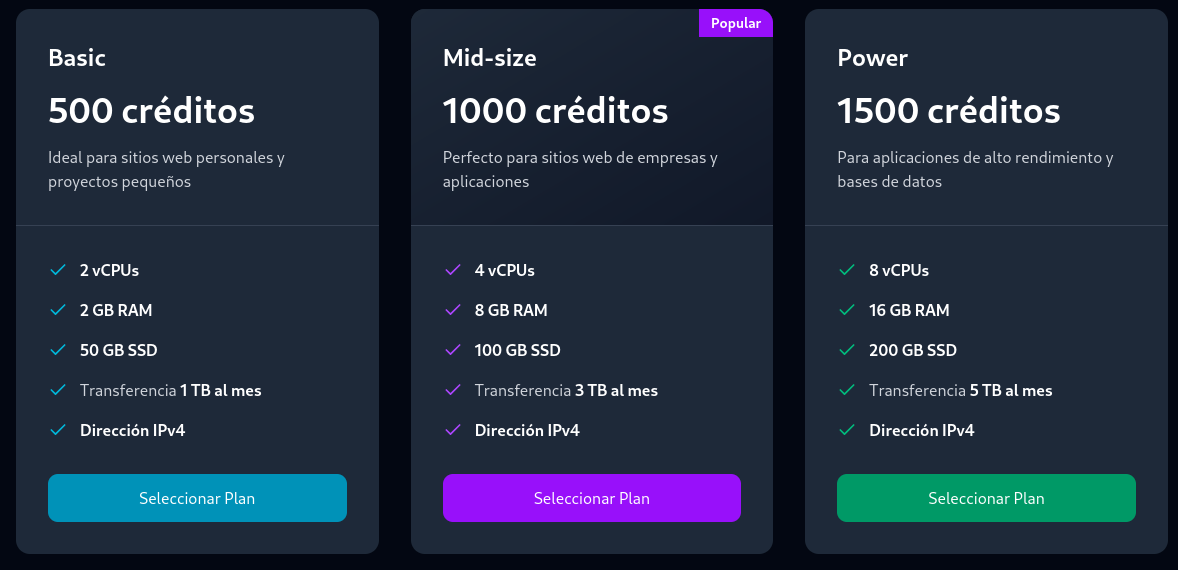
\includegraphics[width=0.9\textwidth]{img/cards.png}
\end{figure}

\newpage
Aquí se muestra el código para mostrar los planes:
\begin{verbatim}
      <section className="py-16">
        <div className="container mx-auto px-4">
          <div className="max-w-6xl mx-auto">
            <div className="grid md:grid-cols-3 gap-8">
              {plans.map((plan) => {
                const style = planStyles[plan.name as keyof typeof planStyles]
                return (
                  <PlanCard 
                    key={plan.id}
                    plan={plan}
                    style={style}
                    onSelect={handleSelectPlan}
                  />
                )
              })}
            </div>
          </div>
        </div>
      </section>
\end{verbatim}

Como se puede apreciar, solo se llama al componente en lugar de todo el código necesario para mostrarlo.

Todos los datos de los planes se obtienen de la base de datos a través del \textit{backend}, lo que permite una fácil actualización y gestión de los planes disponibles.

Para el desarrollo del frontend, he usado el servidor integrado de Vite, el cual se lanza con el siguiente comando:
\begin{verbatim}
    npm run dev
\end{verbatim} 
Esto inicia un servidor de desarrollo que permite ver los cambios en tiempo real mientras se desarrolla la aplicación.

De cara al despliegue en producción, he utilizado Docker para hacer una imagen de la aplicación con un \textit{build multi-stage}, lo que permite crear un contenedor para construir el fichero final de frontend, mientras que el segundo contenedor (nginx) sirve el contenido estático generado por el primer contenedor. Más detalles en la sección de Docker.

Todo el código se encuentra en el Anexo A.
\newpage
\blankpage
El siguiente diagrama de flujo muestra las acciones que se pueden realizar desde el frontal:

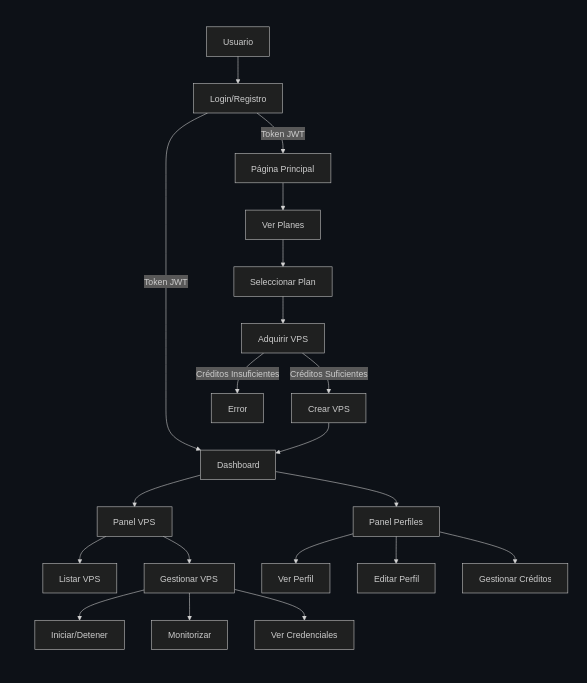
\includegraphics[width=15cm]{img/diagrama_cliente.png}

El cliente tendrá que registrarse para realizar cualquier acción distinta de ver los planes. Una vez registrado, podrá adquirir un VPS, editar su perfil, ver los detalles de su VPS, etc.

\newpage
\blankpage

\newsection{Implementación Backend}
El servidor backend no está expuesto al usuario directamente, se accede por un proxy inverso configurado en el frontend.

Para empezar con el desarrollo del backend, he creado un nuevo proyecto de Node.js con Express utilizando el siguiente comando:
\begin{verbatim}
    npm init -y
    npm install express cors dotenv mariadb bcrypt jsonwebtoken
\end{verbatim}

A partir de aquí, he creado un fichero \textit{server.js} que contiene la configuración básica del servidor Express para su ejecución. Este fichero es el punto de entrada de la aplicación y se encarga de configurar las rutas, middleware y la conexión a la base de datos; escritas en otros ficheros.

Después, he creado diferentes directorios para organizar el código:
\begin{verbatim}
    mkdir routes controllers config middleware
\end{verbatim} 

Como sus nombres rezan, cada directorio tiene una función específica:
\begin{itemize}
    \item \textbf{routes}: Contiene los archivos de rutas que definen los endpoints de la API.
    \item \textbf{controllers}: Contiene la lógica de negocio para cada endpoint, separando la lógica de las rutas.
    \item \textbf{config}: Contiene la configuración de la base de datos y otros parámetros del servidor.
    \item \textbf{middleware}: Contiene la lógica de autenticación a través de JWT.
\end{itemize}

Los datos de conexión a BBDD, en el directorio \textit{config}, los aporta Docker por medio de variables de entorno, lo que permite una fácil configuración y despliegue en diferentes entornos.

Adjunto un diagrama de flujo que muestra las acciones que se pueden realizar desde el backend:
\begin{center}
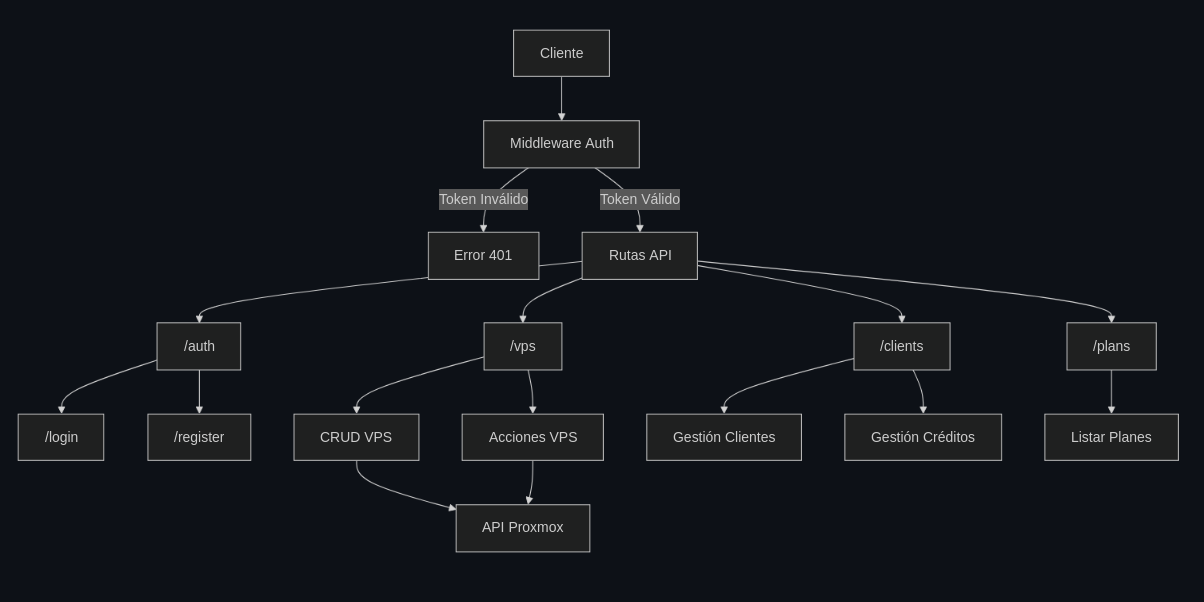
\includegraphics[width=14cm]{img/diagrama_backend.png}
\end{center}

Todas las acciones implican interacción con la base de datos, ya sea para crear un usuario, autenticarlo, obtener los planes disponibles o gestionar los VPS del usuario.

\newpage
\blankpage

\newsection{Estructura de la Base de Datos}
La base de datos se ha diseñado para almacenar la información necesaria para gestionar los VPS y los usuarios. La estructura incluye las siguientes tablas:

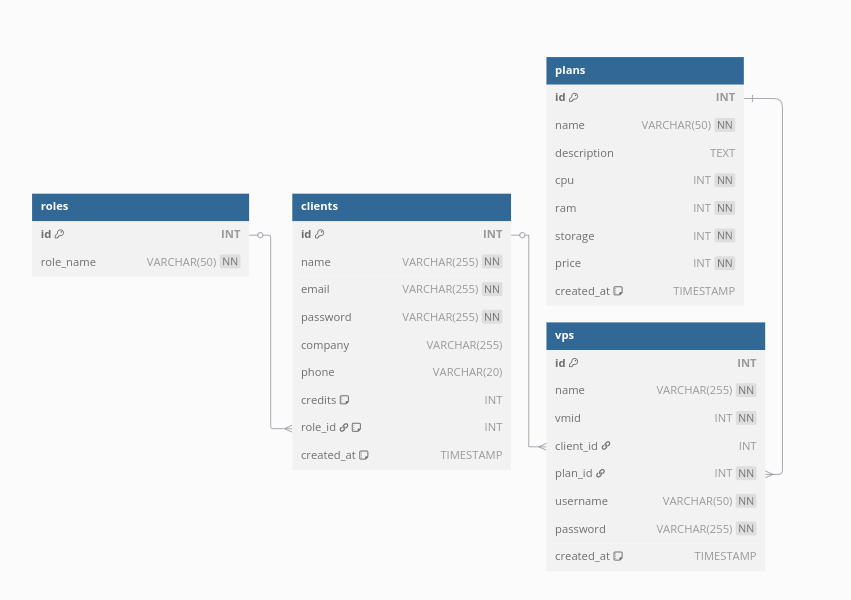
\includegraphics[width=\textwidth]{img/esquema_bd.png}

En el Anexo A se podrá ver el código SQL para crear las tablas y sus relaciones.

\newpage
\blankpage

\newsection{API Proxmox}
Este es el núcleo del proyecto, puesto que esta API es la que interactúa directamente con el hipervisor Proxmox para gestionar los VPS, lo que permite versatilidad para usarla en otros proyectos o incluso para crear un panel de control personalizado.

Para empezar con el desarrollo de la API de Proxmox, he creado un nuevo proyecto de Python con FastAPI en un entorno virtual utilizando los siguientes comandos:
\begin{verbatim}
    python -m venv .venv
    source .venv/bin/activate
    pip install fastapi uvicorn proxmoxer pydantic
\end{verbatim}

He utilizado la libreria \textbf{proxmoxer} para interactuar con la API de Proxmox, así evito tener que lidiar con las peticiones HTTP directamente. Por otro lado, uvicorn es un servidor ASGI que permite ejecutar aplicaciones FastAPI de forma eficiente y el que está a la escucha de las peticiones.

Para este proyecto, dentro del directorio \texttt{app} he creado cuatro directorios principales y un fichero \texttt{main.py} que es el punto de entrada de la aplicación.
\begin{itemize}
    \item \textbf{routes}: Contiene los archivos de rutas que definen los endpoints de la API y la lógica de negocio asociada a cada uno.
    \item \textbf{models}: Contiene los modelos de datos utilizados por Pydantic para validar las entradas y salidas de la API.
    \item \textbf{services}: Contiene funciones auxiliares que no necesariamente son endpoints, pero que se utilizan en la lógica de negocio de las rutas,
    \item \textbf{config}: Contiene la cadena de conexión a Proxmox y otras configuraciones necesarias para la API.
\end{itemize}

Adjunto un diagrama de flujo que muestra las acciones que se pueden realizar desde la API de Proxmox:
\begin{center}
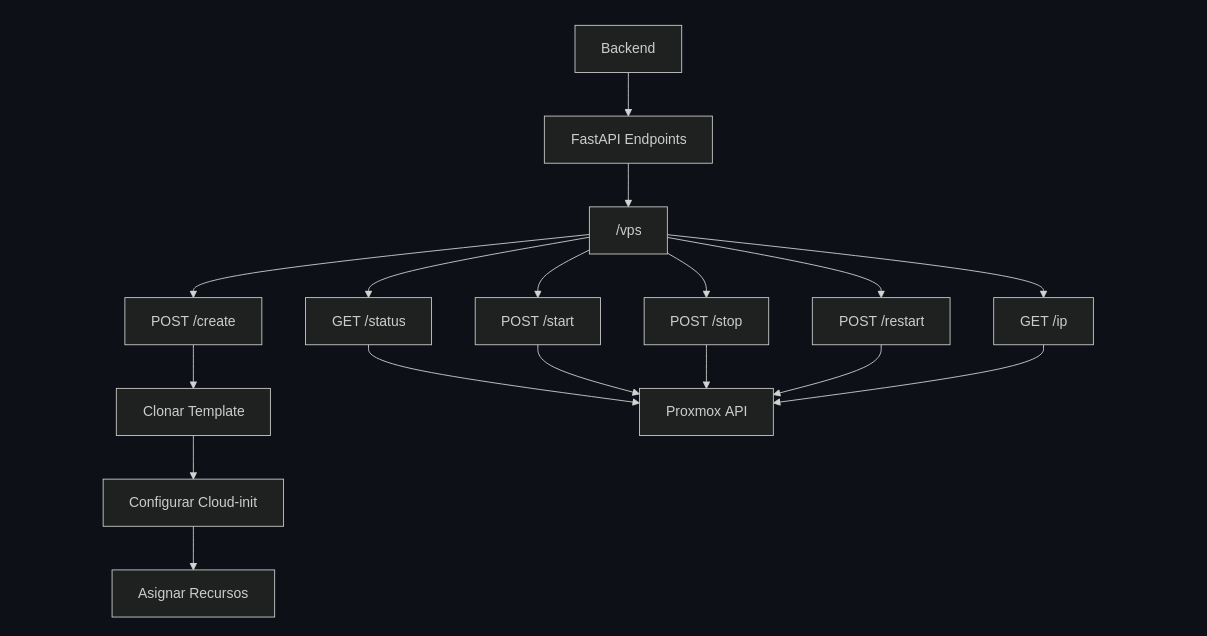
\includegraphics[width=14cm]{img/diagrama_proxmox.png}
\end{center}

En esta API no se valida el origen de la petición ni hay autenticación de usuarios, ya que se supone que solo se va a acceder desde el backend de la aplicación y solo es accesible desde la red interna de Docker. Sin embargo, se valida la entrada de datos en cada endpoint utilizando Pydantic, lo que garantiza que los datos enviados a Proxmox sean correctos y evitar errores.

Cuando se crea una máquina virtual, lo que hace esta API es clonar una plantilla de Proxmox previamente creada, que contiene el sistema operativo y las configuraciones básicas necesarias para el VPS. Para aumentar el almacenamiento se aumenta el tamaño del disco del clon, y de forma automática se incrementan los tamaños de las particiones y del sistema de archivos, para que el usuario pueda usar todo el espacio disponible sin necesidad de realizar ninguna acción adicional. Esto es así por ser una imagen cloud, que ya viene preparada para ser utilizada en entornos de virtualización.

\newpage
\blankpage

\newsection{Imágenes de VPS}
Para crear las imágenes de los VPS, he utilizado scripts de Bash que se ejecutan en el hipervisor Proxmox. Estos scripts descargan las imágenes de los sistemas operativos desde sus fuentes oficiales y las preparan para ser utilizadas como plantillas.

He creado dos scripts, uno para AlmaLinux y otro para Ubuntu, que realizan las siguientes acciones:
\begin{itemize}
    \item Descargan una imagen para cloud del sistema operativo desde su repositorio oficial.
    \item Descomprimen la imagen y la convierten al formato necesario para Proxmox.
    \item Configuran la imagen para que sea compatible con Proxmox, incluyendo la instalación de \texttt{qemu-guest-agent} y la configuración de \texttt{cloud-init}.
\end{itemize}

La elección de estos sistemas operativos se basa en su popularidad y estabilidad, siempre quedando el sistema abierto a incorporar otros sistemas operativos en el futuro.

\newpage
\blankpage

\newchapter{Seguridad}

\newsection{Autenticación y Autorización}
Para garantizar la seguridad de la plataforma, se ha implementado un sistema de autenticación y autorización robusto. Los usuarios deben registrarse y autenticarse para acceder a las funcionalidades del sistema.

El sistema utiliza JWT (JSON Web Tokens) para gestionar las sesiones de usuario. Al iniciar sesión, se genera un token que se envía al cliente y se almacena en el almacenamiento local del navegador. Este token se incluye en las cabeceras de las peticiones a la API para autenticar al usuario.

JWT es un estándar abierto (RFC 7519) que define un formato compacto y autónomo para transmitir información entre partes como un objeto JSON. Este token se firma digitalmente, lo que garantiza su integridad y autenticidad. La información que contiene el token incluye el ID del usuario, la fecha de expiración y otros datos relevantes. En mi caso incluye el rol del usuario.

Las contraseñas de los usuarios se almacenan de forma segura utilizando bcrypt, un algoritmo de hash que protege las contraseñas contra ataques de fuerza bruta. Además, se valida la entrada de datos en todos los endpoints para evitar inyecciones SQL y otros ataques comunes.

\newsection{CORS y Seguridad de la API}
Para proteger la API de accesos no autorizados, se ha configurado CORS (Cross-Origin Resource Sharing) en el servidor Express. Esto permite que solo las solicitudes desde el dominio del frontend sean aceptadas, bloqueando cualquier intento de acceso desde otros orígenes.

CORS es un mecanismo de seguridad que permite o restringe el acceso a recursos web desde diferentes dominios. En este caso, se ha configurado para permitir solo solicitudes desde el dominio del frontend, lo que evita ataques de tipo CSRF (Cross-Site Request Forgery).

\newsection{Seguridad en VPS}
Los VPS creados a través de la plataforma cuentan con varias medidas de seguridad preconfiguradas para proteger los recursos del usuario:
\begin{itemize}
    \item Aislamiento de recursos.
    \item Redes virtuales privadas.
    \item Firewall configurado por defecto.
    \item Actualización automática de plantillas.
\end{itemize}

\newpage
\blankpage
\newchapter{Resultados}
Al finalizar el proyecto, se ha conseguido una plataforma funcional de gestión de VPS que cumple con los objetivos propuestos. La solución permite a los usuarios desplegar y gestionar servidores virtuales de forma sencilla y segura, sin necesidad de conocimientos técnicos avanzados.

\newsection{Interfaz de Usuario}
La interfaz de usuario es intuitiva y fácil de usar, permitiendo a los usuarios gestionar sus VPS de forma eficiente. 

\newsubsection{Inicio}
La página de inicio muestra los planes disponibles y permite a los usuarios registrarse o iniciar sesión.
\begin{figure}[H]
\caption{Página de inicio}
\centering
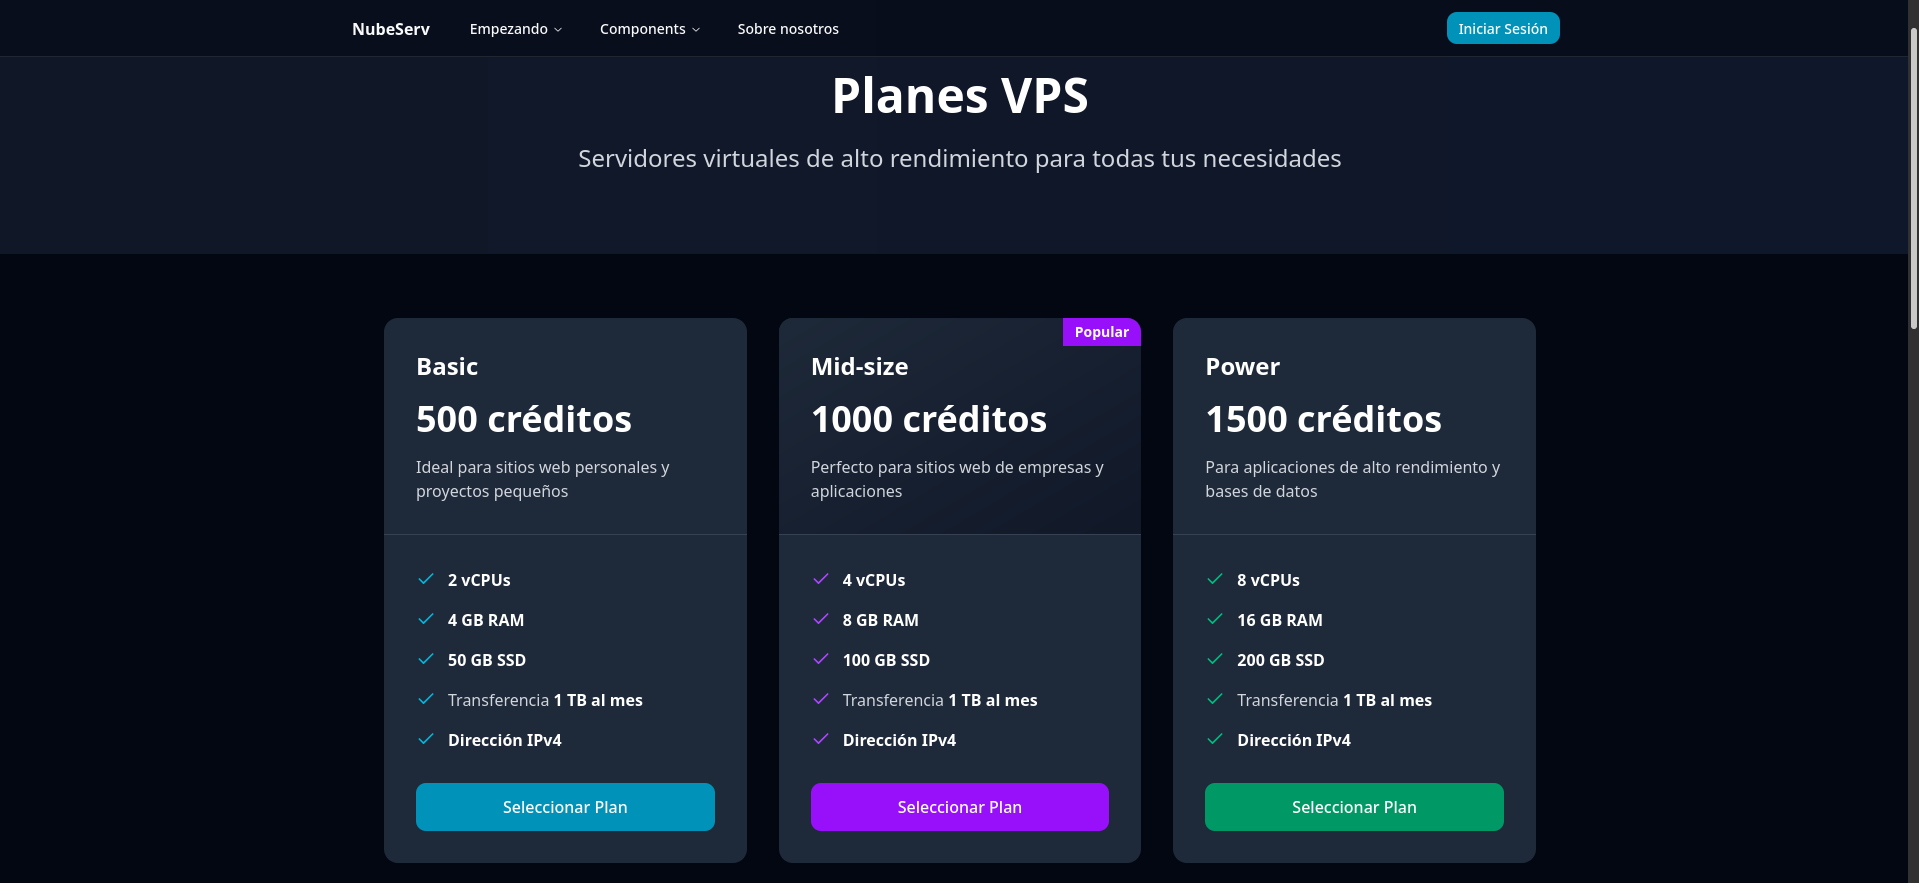
\includegraphics[width=0.9\textwidth]{img/landing.png}
\end{figure}

\newpage
\blankpage

\newsubsection{Página de autenticación}
La página de autenticación permite a los usuarios registrarse o iniciar sesión en la plataforma. El registro requiere un nombre de usuario, correo electrónico y contraseña, mientras que el inicio de sesión solicita solo el correo electrónico y la contraseña.
\begin{figure}[H]
\caption{Formulario de inicio de sesión}
\centering
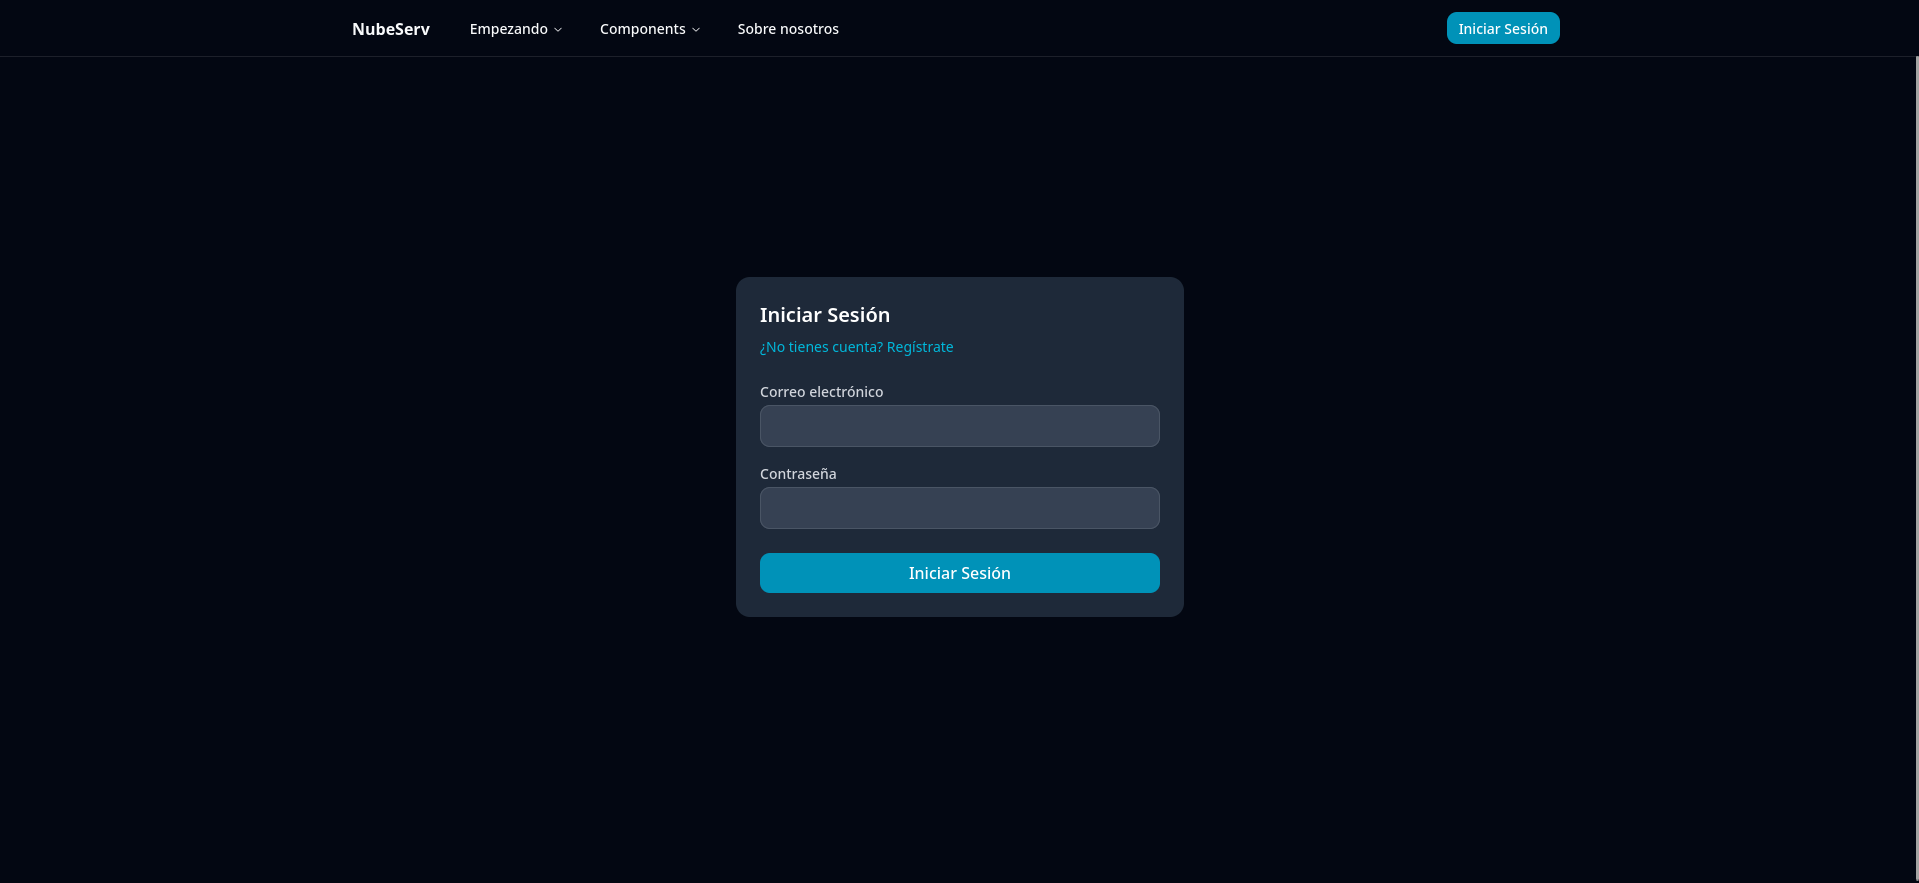
\includegraphics[width=0.9\textwidth]{img/auth_page.png}
\end{figure}
\begin{figure}[H]
\caption{Formulario de registro}
\centering
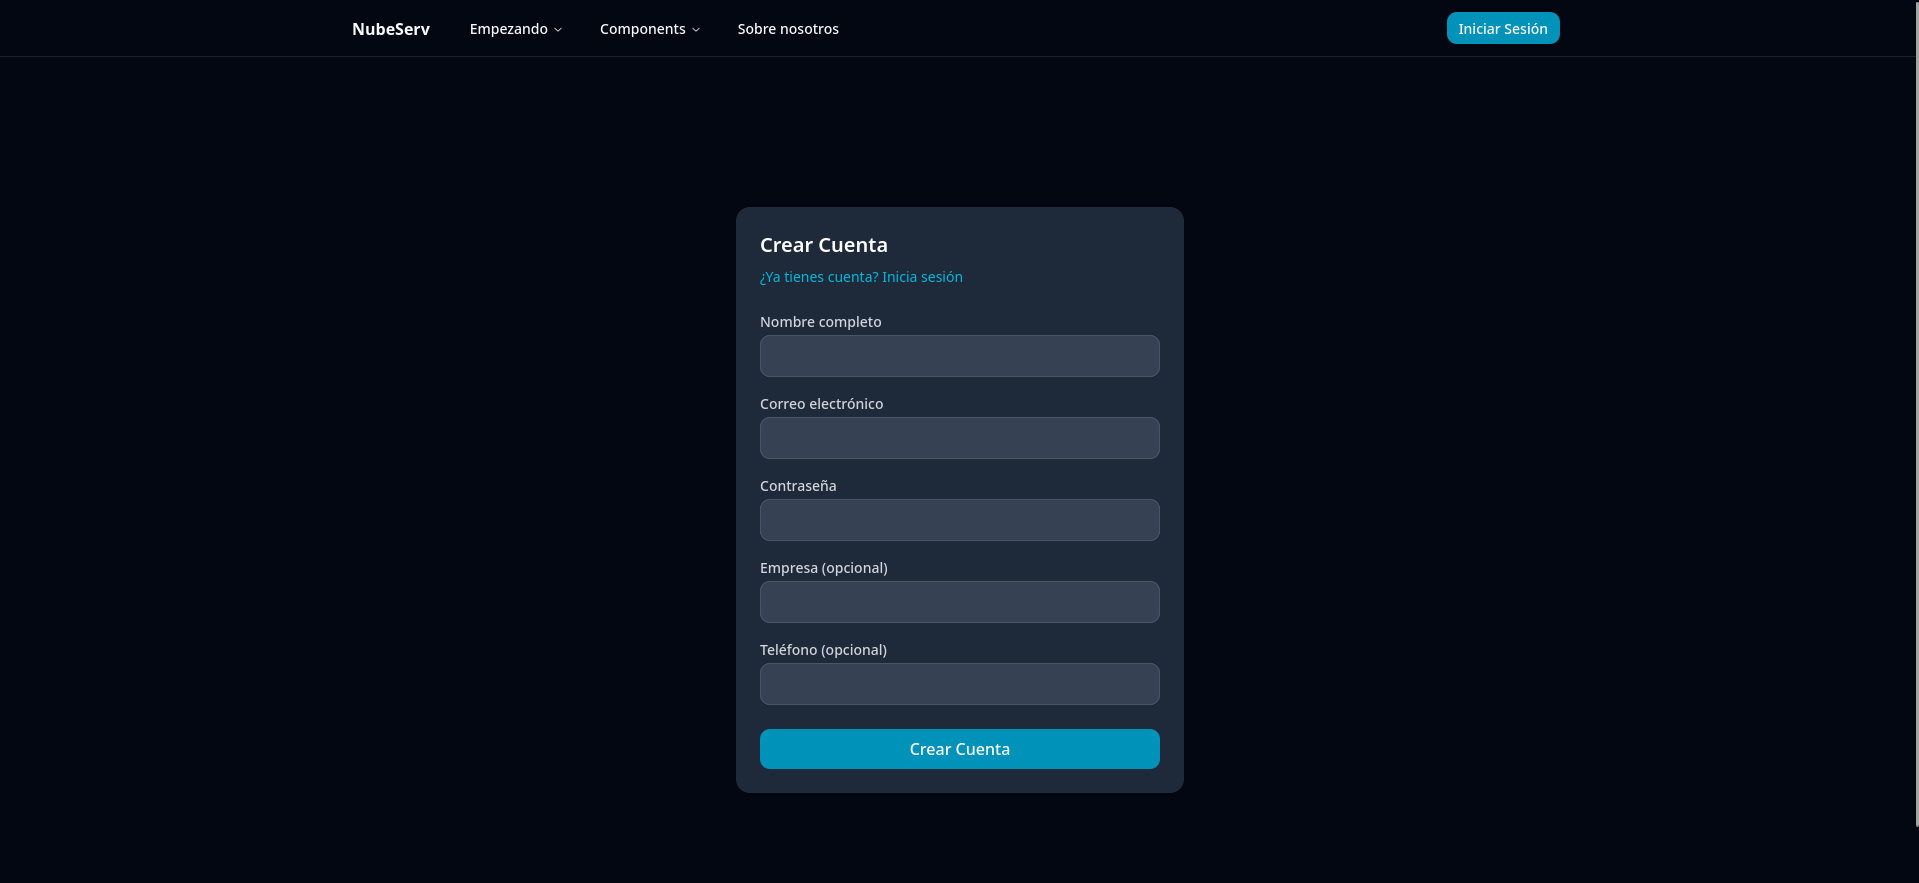
\includegraphics[width=0.9\textwidth]{img/auth_register_page.png}
\end{figure}

\newpage
\blankpage

\newsubsection{Panel de control}
El panel de control muestra los VPS del usuario, permitiendo crear, editar y eliminar servidores virtuales. También se pueden ver los detalles de cada VPS, incluyendo el estado, recursos asignados y acciones disponibles.
\begin{figure}[H]
\caption{Panel de control - Sección de VPS}
\centering
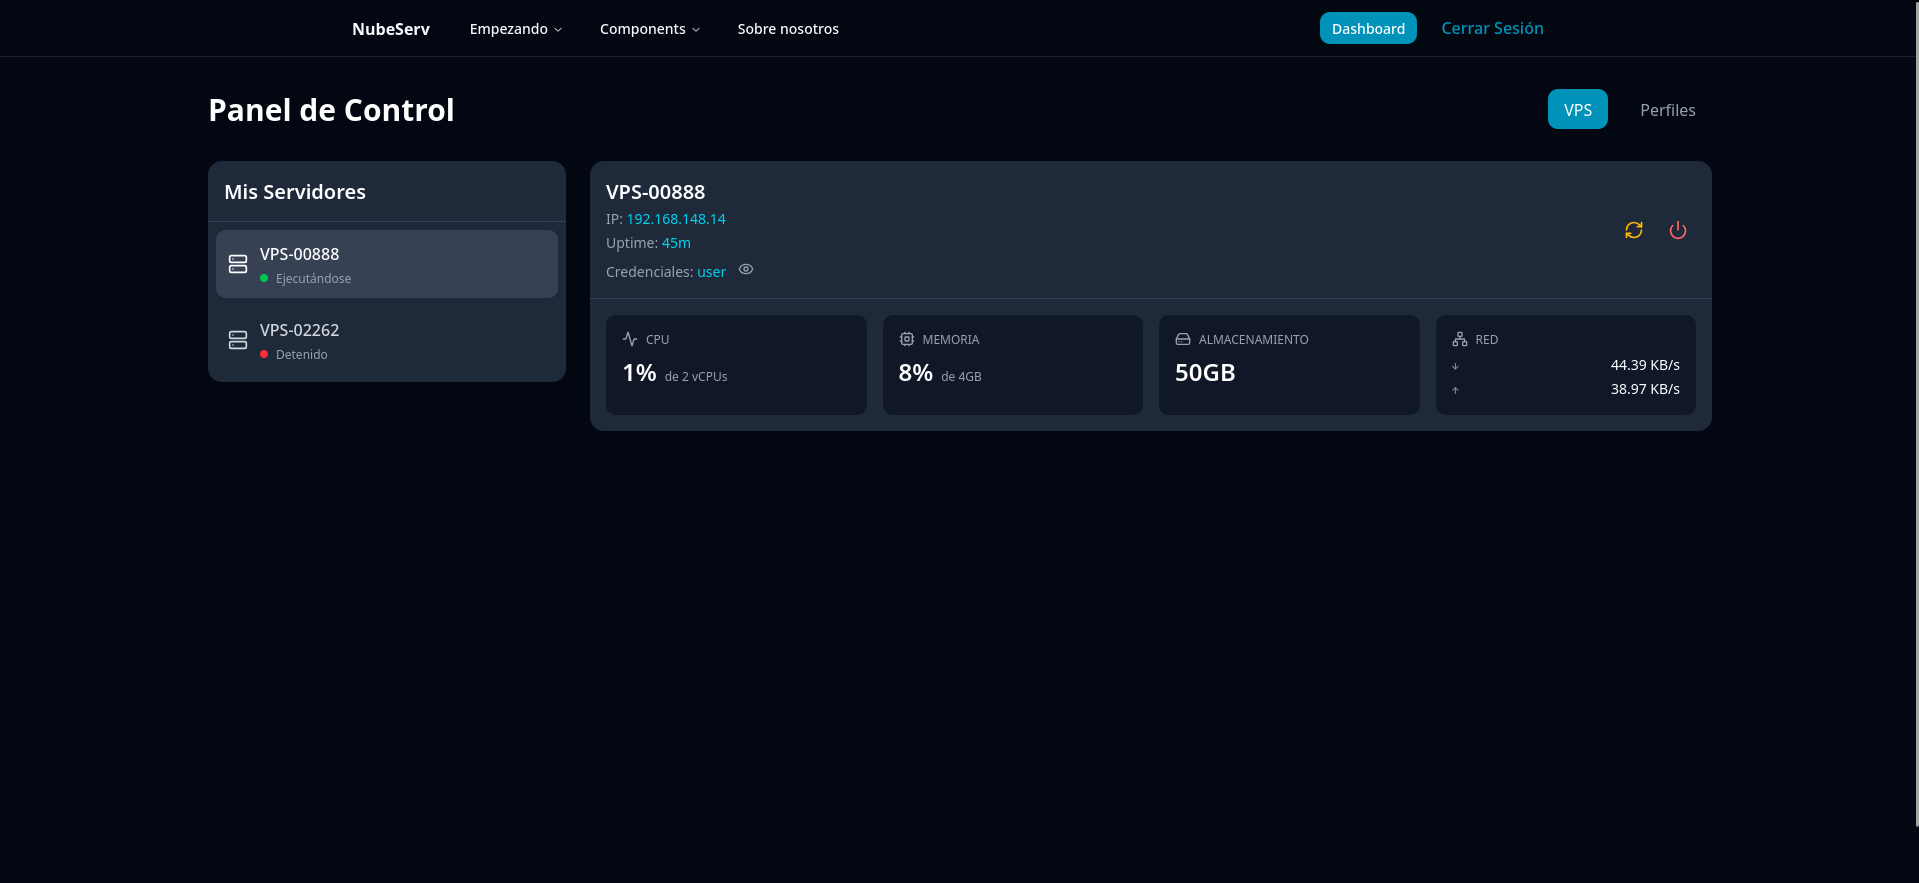
\includegraphics[width=0.9\textwidth]{img/dashboard.png}
\end{figure}
\begin{figure}[H]
\caption{Panel de control - Sección de Perfil}
\centering
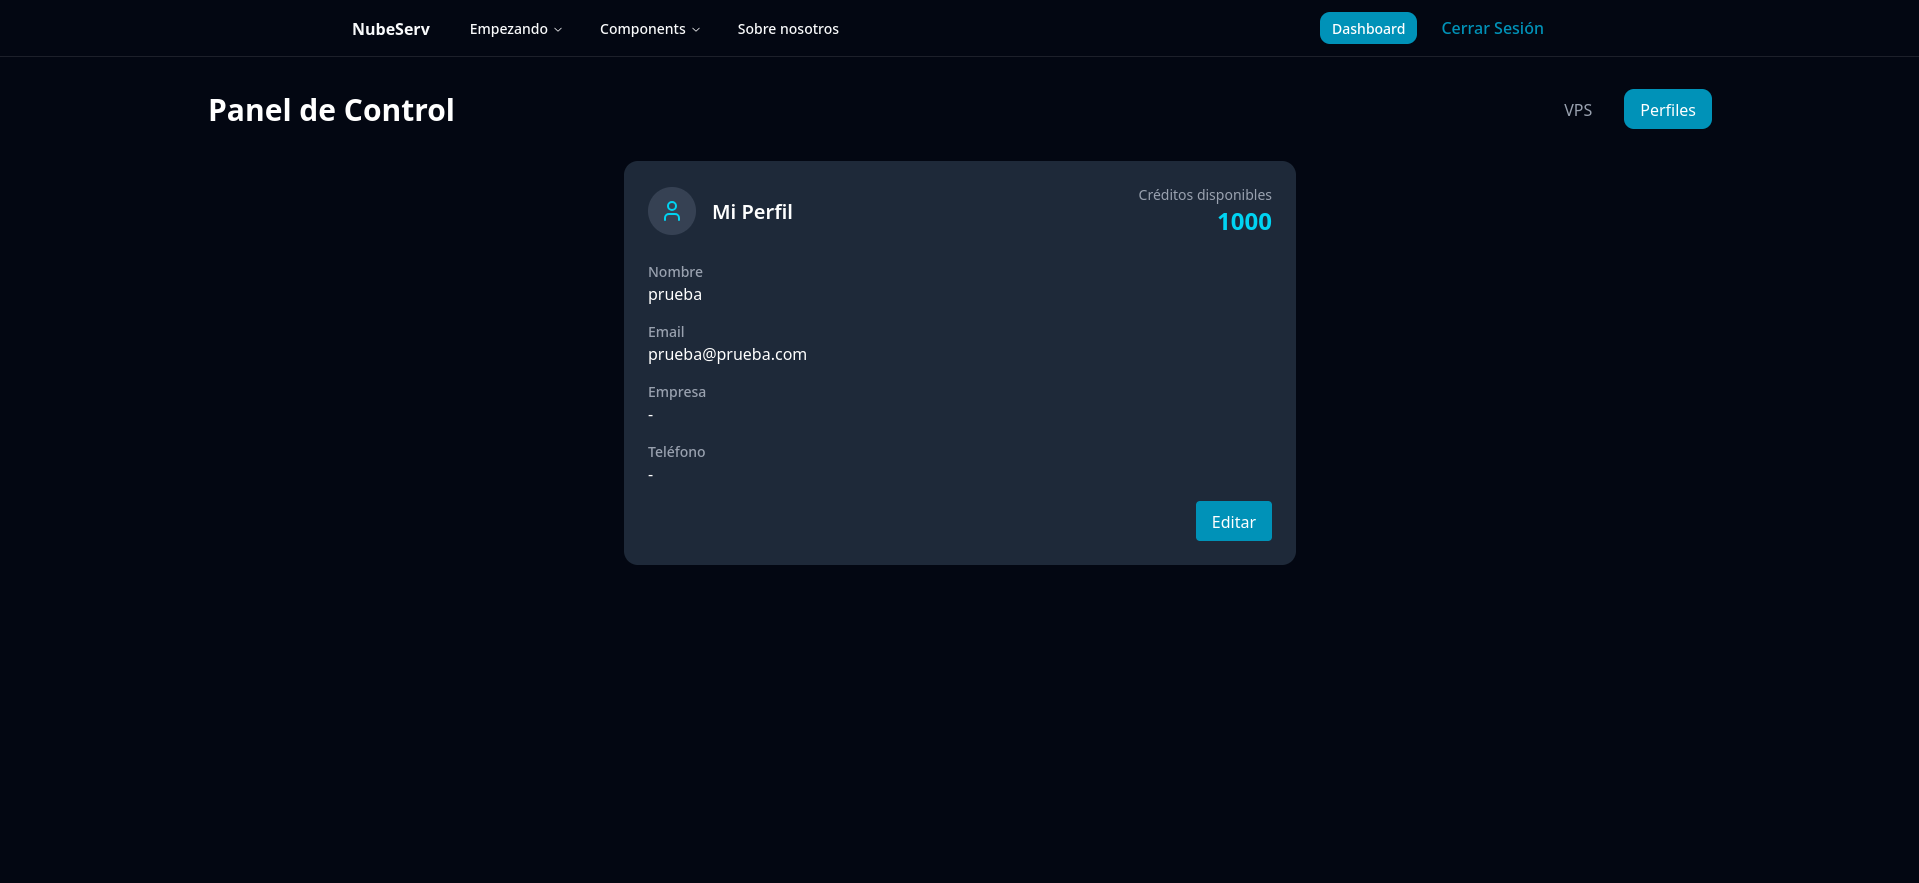
\includegraphics[width=0.9\textwidth]{img/dashboard_profile.png}
\end{figure}

\newpage
\blankpage

\newsection{Creación de VPS}
La creación de un VPS se realiza a través de un formulario que permite seleccionar el plan deseado. Una vez enviado el formulario, se crea el VPS en Proxmox y se muestra en el panel de control del usuario.
\begin{figure}[H]
\caption{Formulario de creación de VPS}
\centering
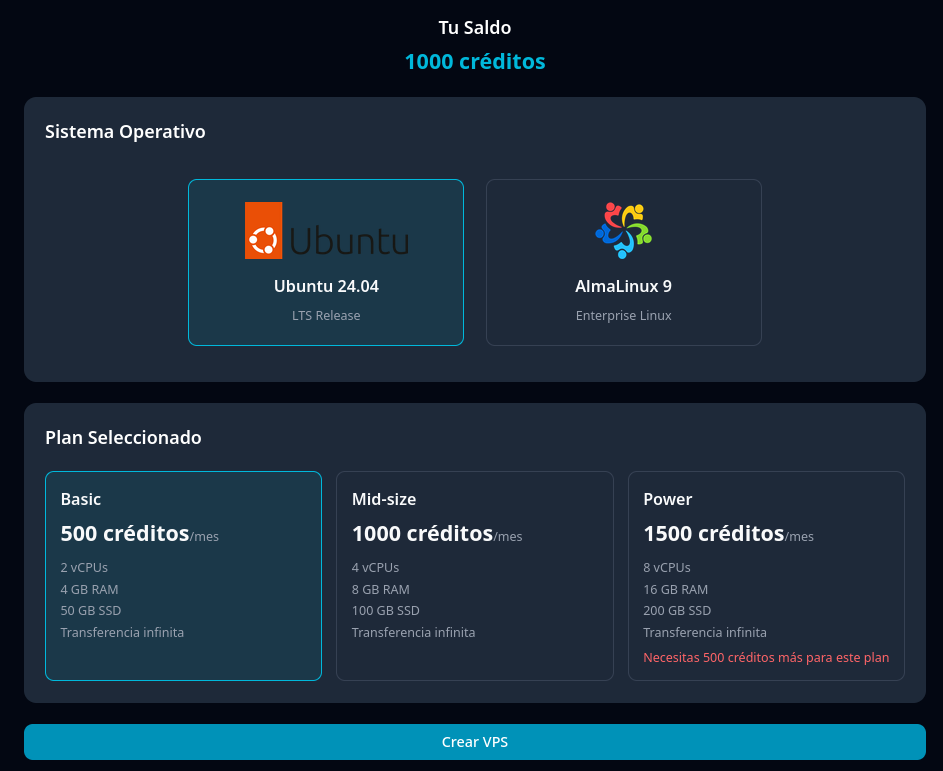
\includegraphics[width=0.9\textwidth]{img/formulario_vps.png}
\end{figure}

\newpage
\blankpage

En Proxmox genera las siguientes acciones, de forma automatizada por una llamada de la API de Express (la de la web) hacia la API de Proxmox (la de Python):
\begin{figure}[H]
\caption{Acciones generadas en Proxmox}
\centering
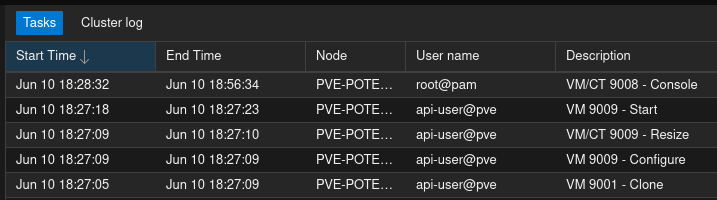
\includegraphics[width=0.9\textwidth]{img/proxmox_tasks.png}
\end{figure}

La acción \textit{configure} asigna la RAM y el número de núcleos:
\begin{figure}[H]
\caption{Acción \textit{configure} en Proxmox}
\centering
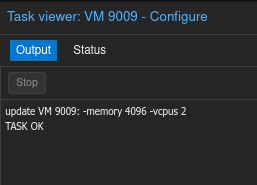
\includegraphics[width=0.4\textwidth]{img/proxmox_configure.png}
\end{figure}

La acción \textit{resize} aumenta el tamaño del disco:
\begin{figure}[H]
\caption{Acción \textit{resize} en Proxmox}
\centering
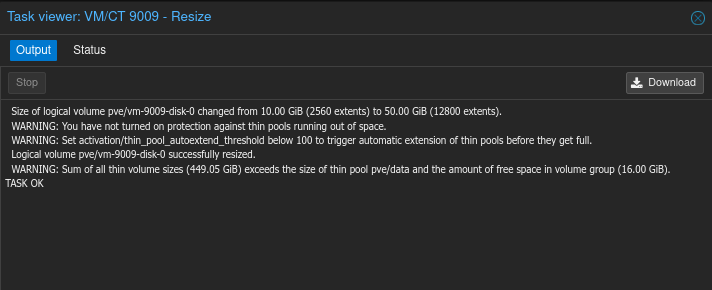
\includegraphics[width=0.9\textwidth]{img/proxmox_resize.png}
\end{figure}

\newpage
\blankpage

\newchapter{Conclusiones y Trabajo Futuro}
\newsection{Conclusiones}
Con este proyecto, he logrado desarrollar una plataforma de \textit{hosting} VPS que permite a los usuarios desplegar y gestionar servidores virtuales de forma sencilla y segura. 

Se ha desplegado con un método fácil de usar, lo que facilita el desarrollo de la aplicación y su publicación.

Ha sido gracias a soluciones de código abierto que he podido desarrollar esta plataforma con facilidad y rapidez, como \textbf{proxmoxer} para interactuar con Proxmox, \textbf{FastAPI} para la API de Proxmox, y \textbf{shadcn/ui} para los componentes del frontend.

\newsection{Trabajo Futuro}
De cara al futuro, y si hubiera más tiempo, se podrían implementar las siguientes mejoras:
\begin{itemize}
    \item \textbf{Soporte para más sistemas operativos}: Ampliar la plataforma para incluir otros sistemas operativos como Debian, Fedora, Windows Server, etc., lo que aumentaría la versatilidad de la solución.
    \item \textbf{Sistema de copias de seguridad}: Con Proxmox Backup Server se puede implementar muy rápidamente un sistema robusto de copias de seguridad.
    \item \textbf{Métricas avanzadas con histórico}: Ahora mismo solo se muestran las métricas actuales de CPU, RAM y disco, pero se podría implementar un sistema de monitorización más avanzado que permita ver el histórico de uso de recursos y alertas con Zabbix.
    \item \textbf{Soporte para múltiples hipervisores}: Ampliar la plataforma para soportar otros hipervisores como vSphere, KVM, Nutanix, etc., lo que aumentaría la versatilidad de la solución.
    \item \textbf{Personalización del VPS}: Posibilidad de que el usuario inserte su usuario, contraseña y clave SSH en el formulario de creación.
\end{itemize}

\newpage
\blankpage

\newchapter{Bibliografía}
\begin{itemize}
    \item \textbf{React}: https://reactjs.org/
    \item \textbf{FastAPI}: https://fastapi.tiangolo.com/
    \item \textbf{Proxmox}: https://pve.proxmox.com/wiki/
        \subitem - \textbf{Proxmox VE API Documentation}: https://pve.proxmox.com/pve-docs/api-viewer/
    \item \textbf{Express - Node.js web application framework}: https://expressjs.com/
    \item \textbf{Documentation - MariaDB.org}: https://mariadb.org/documentation/
    \item \textbf{Build your Component Library - shadcn/ui}: https://ui.shadcn.com/
    \item \textbf{Get started with Tailwind CSS}: https://tailwindcss.com/docs
    \item \textbf{Docker Docs}: https://docs.docker.com/
    \item Manhas Mansi. How To Use An .env File In Docker Compose.
    \subitem https://www.warp.dev/terminus/docker-compose-env-file
\end{itemize}
\end{document}